% !TEX root = main.tex
\chapter{Systematic uncertainties}
\label{ch:systeamticUncerts}

Systematic uncertainties are estimated in several ways.
First, parameters are constraint by means of Gaussian functions in various steps of the analysis and the influence of these constraints on the resulting uncertainties has to be estimated (\cref{sec:SystUncertsGauss}).
Second, pseudoexperiments are used to test the systematic effects of certain assumptions such as $\DG=0$ (\cref{sec:systUncertsPseudo}).
Finally, systematic effects related to the mass model and the associated determination of the \emph{sWeights} are also determined (\cref{sec:SystUncertMass}).

Again it should be stressed that all work in this chapter related to the mass fit was done by a collaborator.
This includes parts of the estimated uncertainties in \cref{sec:SystUncertsGauss} and the estimations presented in \cref{sec:SystUncertMass}.

Table \ref{tab:SystUncertsFull} shows a list of all effects investigated.
The total uncertainty is calculated from the sum of the squared individual contributions.

\begin{table}[tbp]
	\centering
	\caption{Systematic uncertainties on the \CP parameters \Sf and \Sfbar listed by decreasing order.
	The \enquote{fit biases} are the residuals of the fits to bootstrapped simulated candidates described in \cref{sec:valOnSim}.
	The total uncertainty is calculated from the sum of the squared individual contributions.}
	\begin{tabular}{lS[table-format=1.4]S[table-format=1.4]}
		\toprule
		Source & \Sf & \Sfbar\\
		\midrule
		uncertainty of \dm 						& 0.0073 & 0.0061 \\
		fit biases 								& 0.0068 & 0.0018 \\
		background subtraction 					& 0.0042 & 0.0023 \\
		flavour-tagging models 					& 0.0011 & 0.0015 \\
		flavour-tagging efficiency asymmetries 	& 0.0012 & 0.0015 \\
		decay-time resolution 					& 0.0012 & 0.0008 \\
		\dllkpi efficiencies 					& 0.0008 & 0.0008 \\
		acceptance model 						& 0.0007 & 0.0007 \\
		assumption on \DG 						& 0.0007 & 0.0007 \\
		assumption on \Cf and \Cfbar 			& 0.0006 & 0.0006 \\
		\midrule
		total 									& 0.0111 & 0.0073 \\
		\midrule
		statistical uncertainties 				& 0.0198 & 0.0199 \\
		\bottomrule
	\end{tabular}
	\label{tab:SystUncertsFull}
\end{table}


\section{Systematic uncertainties from Gaussian constraints}
\label{sec:SystUncertsGauss}

Gaussian constraints have been used in two places of the analysis.
On the one hand, external measurements of the \Bz oscillation frequency \dm and the \Bz lifetime $\tau$ are used and implemented by such constraints in the decay-time fit.
On the other hand, the uncertainties of the efficiencies of the \dllkpi cuts in \cref{ch:massfit} are propagated through constraints by means of Gaussian functions in the mass fit.
This second uncertainty was calculated by a collaborator and the procedure is described shortly for completeness.

In order to investigate the composition of the uncertainties of \Sf and \Sfbar in the decay-time fit, the constrained parameters are set to the central value of the Gaussian constraint to obtain the purely statistical uncertainty.
These purely statistical uncertainties are \num{0.0198} and \num{0.0199} for \Sf and \Sfbar respectively, with a correlation of \SI{60}{\percent}.
From the difference of the squared uncertainties with and without constraint, the systematic uncertainty on the corresponding parameter is then obtained.
For \dm this results in a fully anticorrelated systematic uncertainty of \num{0.0073} and \num{0.0061} for \Sf and \Sfbar, respectively.
The systematic uncertainty for the \Bz lifetime $\tau$ is negligible.

The efficiency of the requirement on \dllkpi depends on the binning of several observables used in the determinaton of the \dllkpi.
This effect is refleceted in the uncertainties of the efficiency which are further propagated to the mass fit by Gaussian constraints.
The mass fit is repeated with the \dllkpi requirement efficiencies fixed to the mean value of the Gaussian constraint.
The resulting \emph{sWeights} are then used in an alternative decay-time fit to extract the \CP parameters.
The difference in quadrature between the result for \Sf and \Sfbar of the nominal fit and this alternative fit is used as systematic uncertainty.
It follows an uncertainty of \num{0.0008} for both, \Sf and \Sfbar.

\section{Estimations with pseudoexperiments}
\label{sec:systUncertsPseudo}

Systematic uncertainties are determined using pseudoexperiments by generating data samples of the same size as the \BdToDpi signal yield.
In this generation all parameters are set to the values found in the nominal decay-time fit, except for \Sf and \Sfbar.
In order to prevent observer bias, the analysis was performed blind for these parameters and therefore the values used in the generation of the simulated events are adopted for \Sf and \Sfbar.
For each pseudoexperiment in the generation the PDF from \cref{eq:FinalDecayTimePDF} is modified with alternate models, corresponding to the various assumptions which are made in the analysis and fitted back with the nominal model.
Each study consists of \num{1000} pseudoexperiments for which the distribution of residuals of \Sf and \Sfbar are studied, whereby the residual is defined as the difference between the generation value and the fitted value.
Like in \cref{sec:valOnSim}, this residual distributions are fitted with Gaussian functions.
The deviation from zero of the mean value of this function is taken as systematic uncertainty; if the mean value is compatible within one standard deviation with zero, the error on the mean is taken as systematic uncertainty.
In this way, uncertainties are determined for the flavour tagging calibration model, the acceptance model, the decay-time resolution and the assumptions on \DG and \Cf.

\subsection*{Flavour tagging calibration model}

For the SS taggers the nominal model with a first-order polynomial is used in the generation while the model for the OS taggers is reduced by one degree compared to the nominal one.
In the fit, the polynomials of the calibration models are then increased by one degree for both types of tagging algorithms, compared to what is used during generation. Figure \ref{fig:systUncertFTmodel} shows the distribution of residuals. The systematic uncertainty is \num{0.0011} and \num{0.0015} for \Sf and \Sfbar, respectively.
\begin{figure}[tbp]
    \centering
    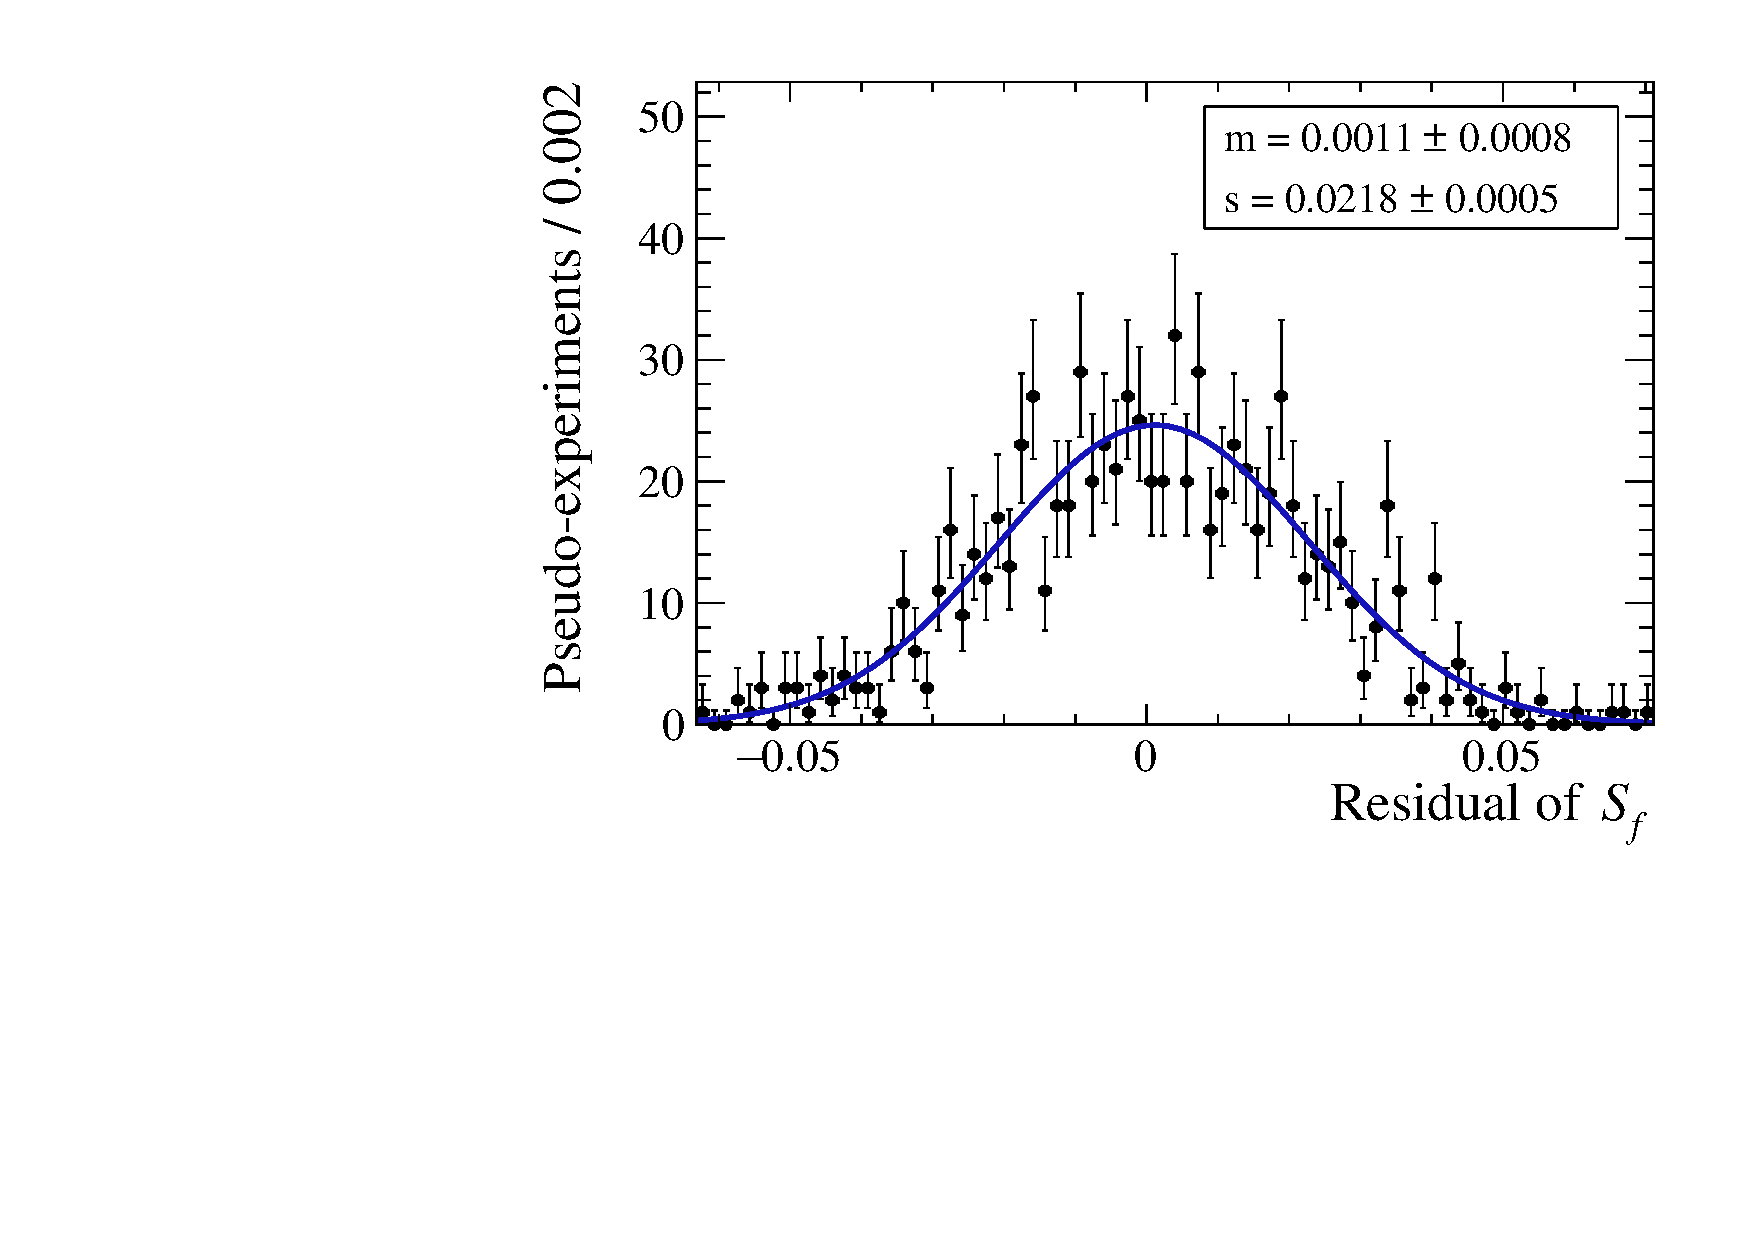
\includegraphics[width=0.48\textwidth]{10Systematics/figs/FT_Sf_res.pdf}
    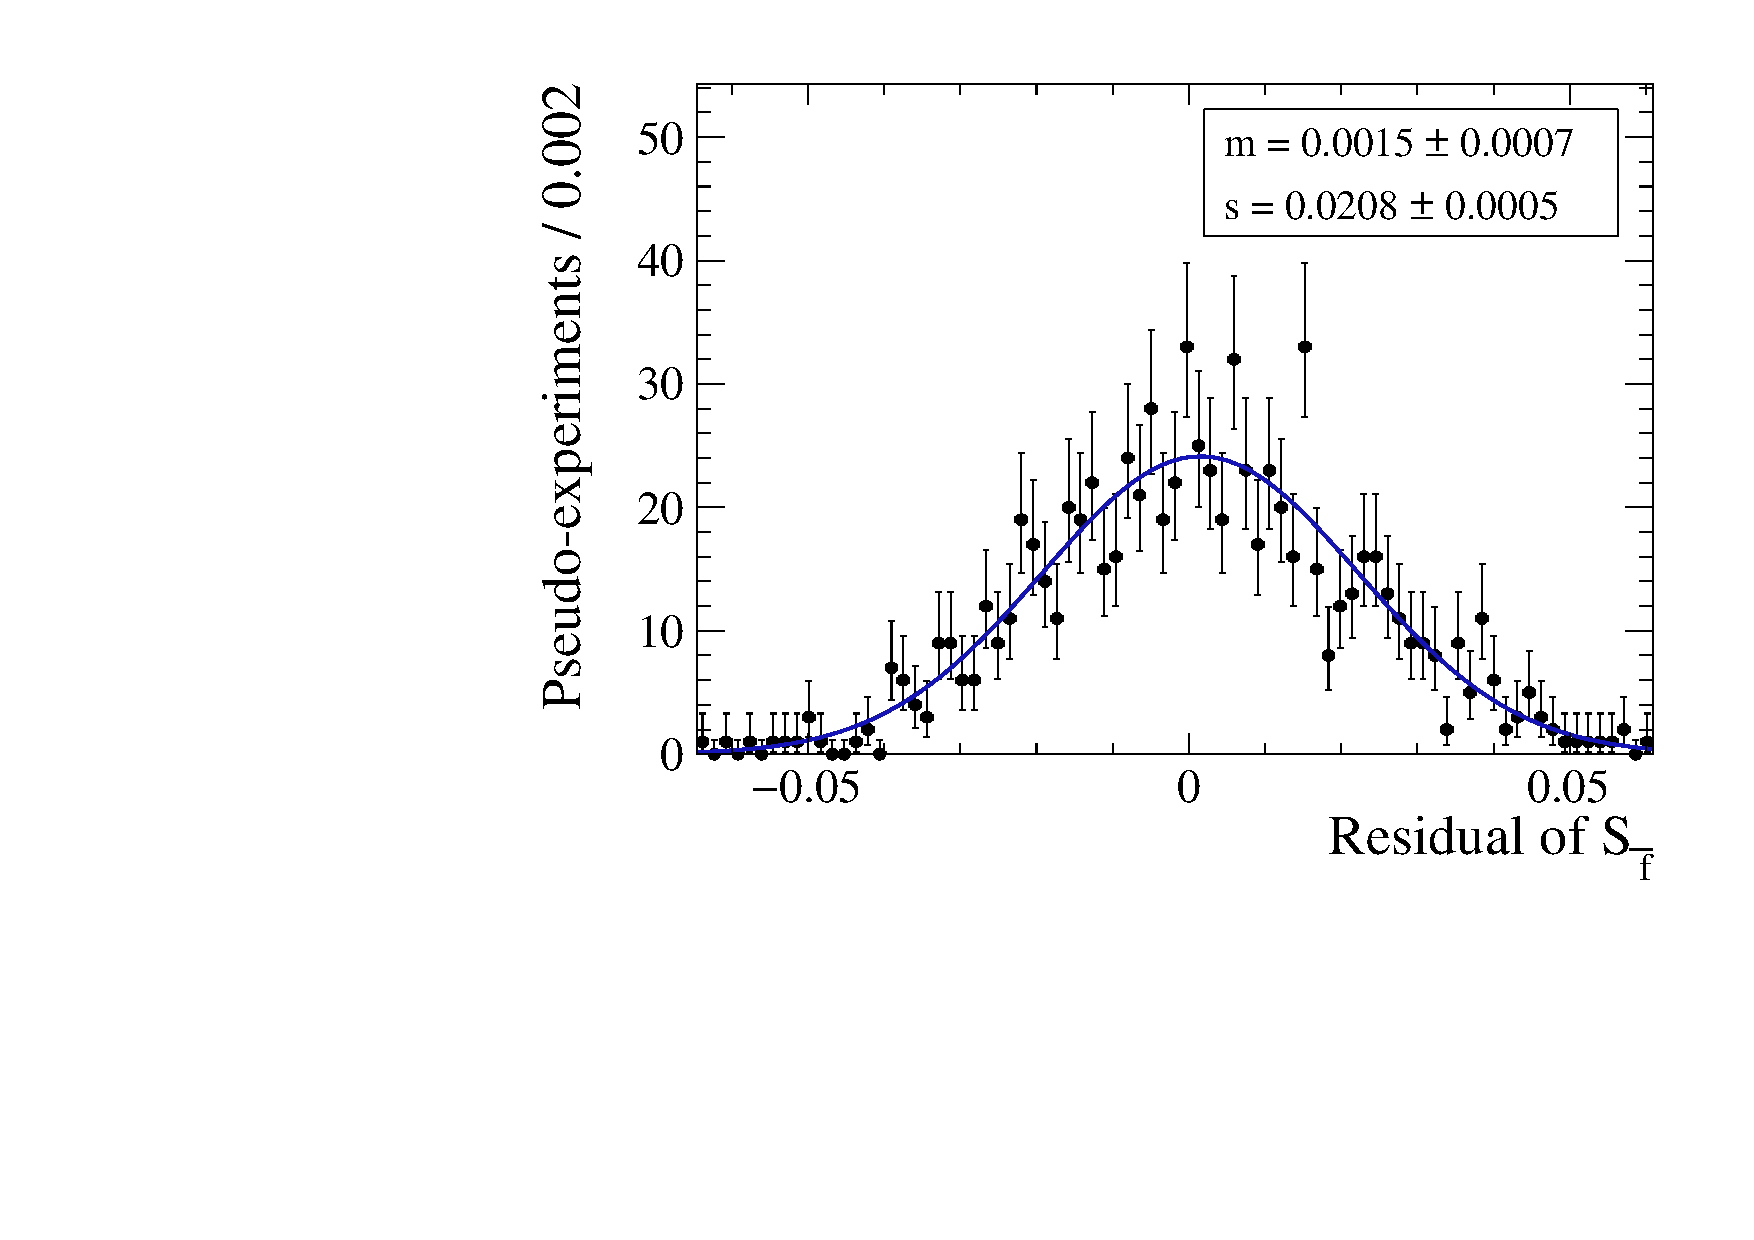
\includegraphics[width=0.48\textwidth]{10Systematics/figs/FT_Sfbar_res.pdf}
    \caption{Distribution of residuals for \Sf (left) and \Sfbar (right) to determine the systematic uncertainty due to the flavour tagging calibration model.}
    \label{fig:systUncertFTmodel}
\end{figure}

\subsection*{Decay-time resolution}

Two different sets of samples are generated to determine the systematic uncertainty due to the decay-time resolution, the first with an average resolution \SI{20}{\femto\second} higher than the nominal resolution of \SI{54.91}{\femto\second}, the second with an average resolution \SI{20}{\femto\second} lower than the nominal one.
In both cases the nominal resolution is used in the fit.
The residual distributions of both studies are shown in \cref{fig:systUncertRes}.
The larger uncertainty resulting from the two studies for \Sf and \Sfbar is then chosen as systematic uncertainty.
The result is \num{0.0012} and \num{0.0008} for \Sf and \Sfbar, respectively.
\begin{figure}[tbp]
    \centering
    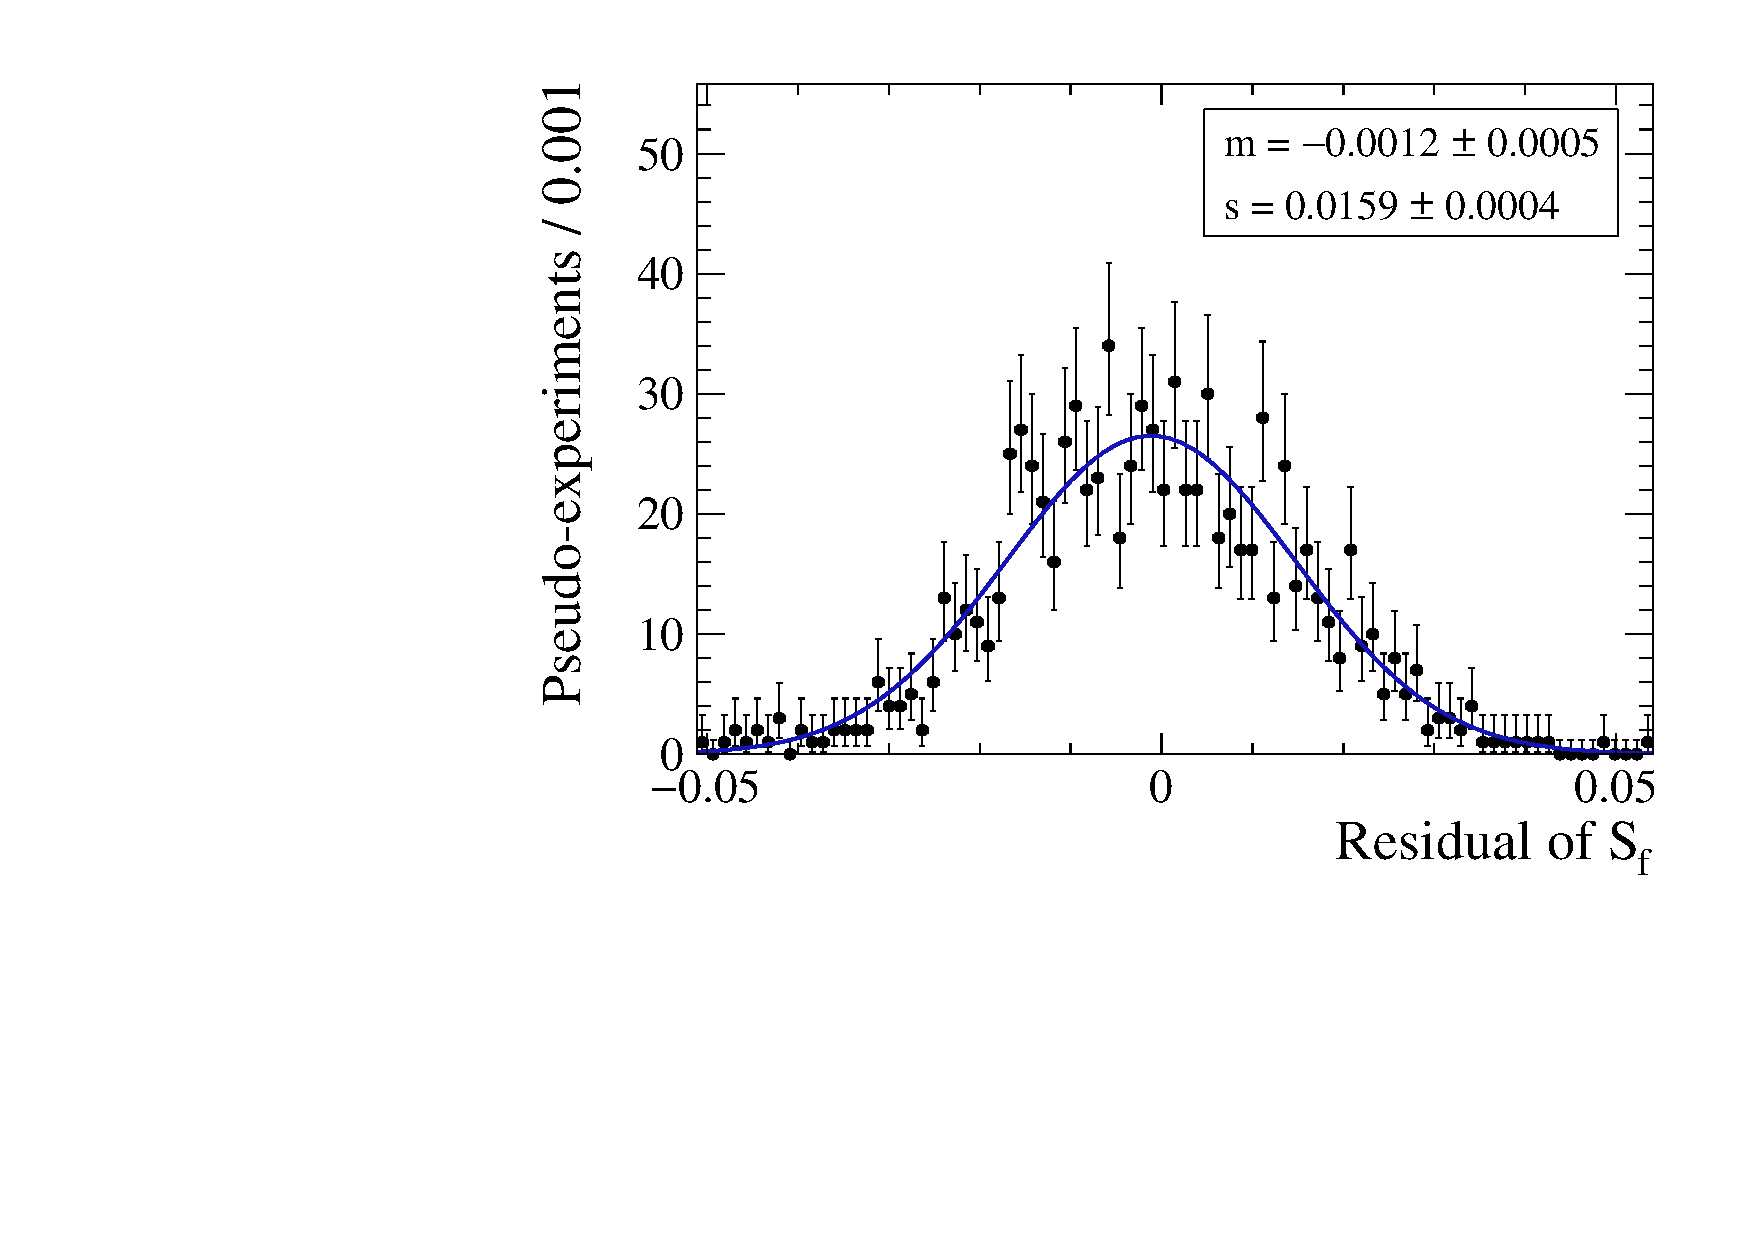
\includegraphics[width=0.48\textwidth]{10Systematics/figs/ResHigh_Sf_res.pdf}
    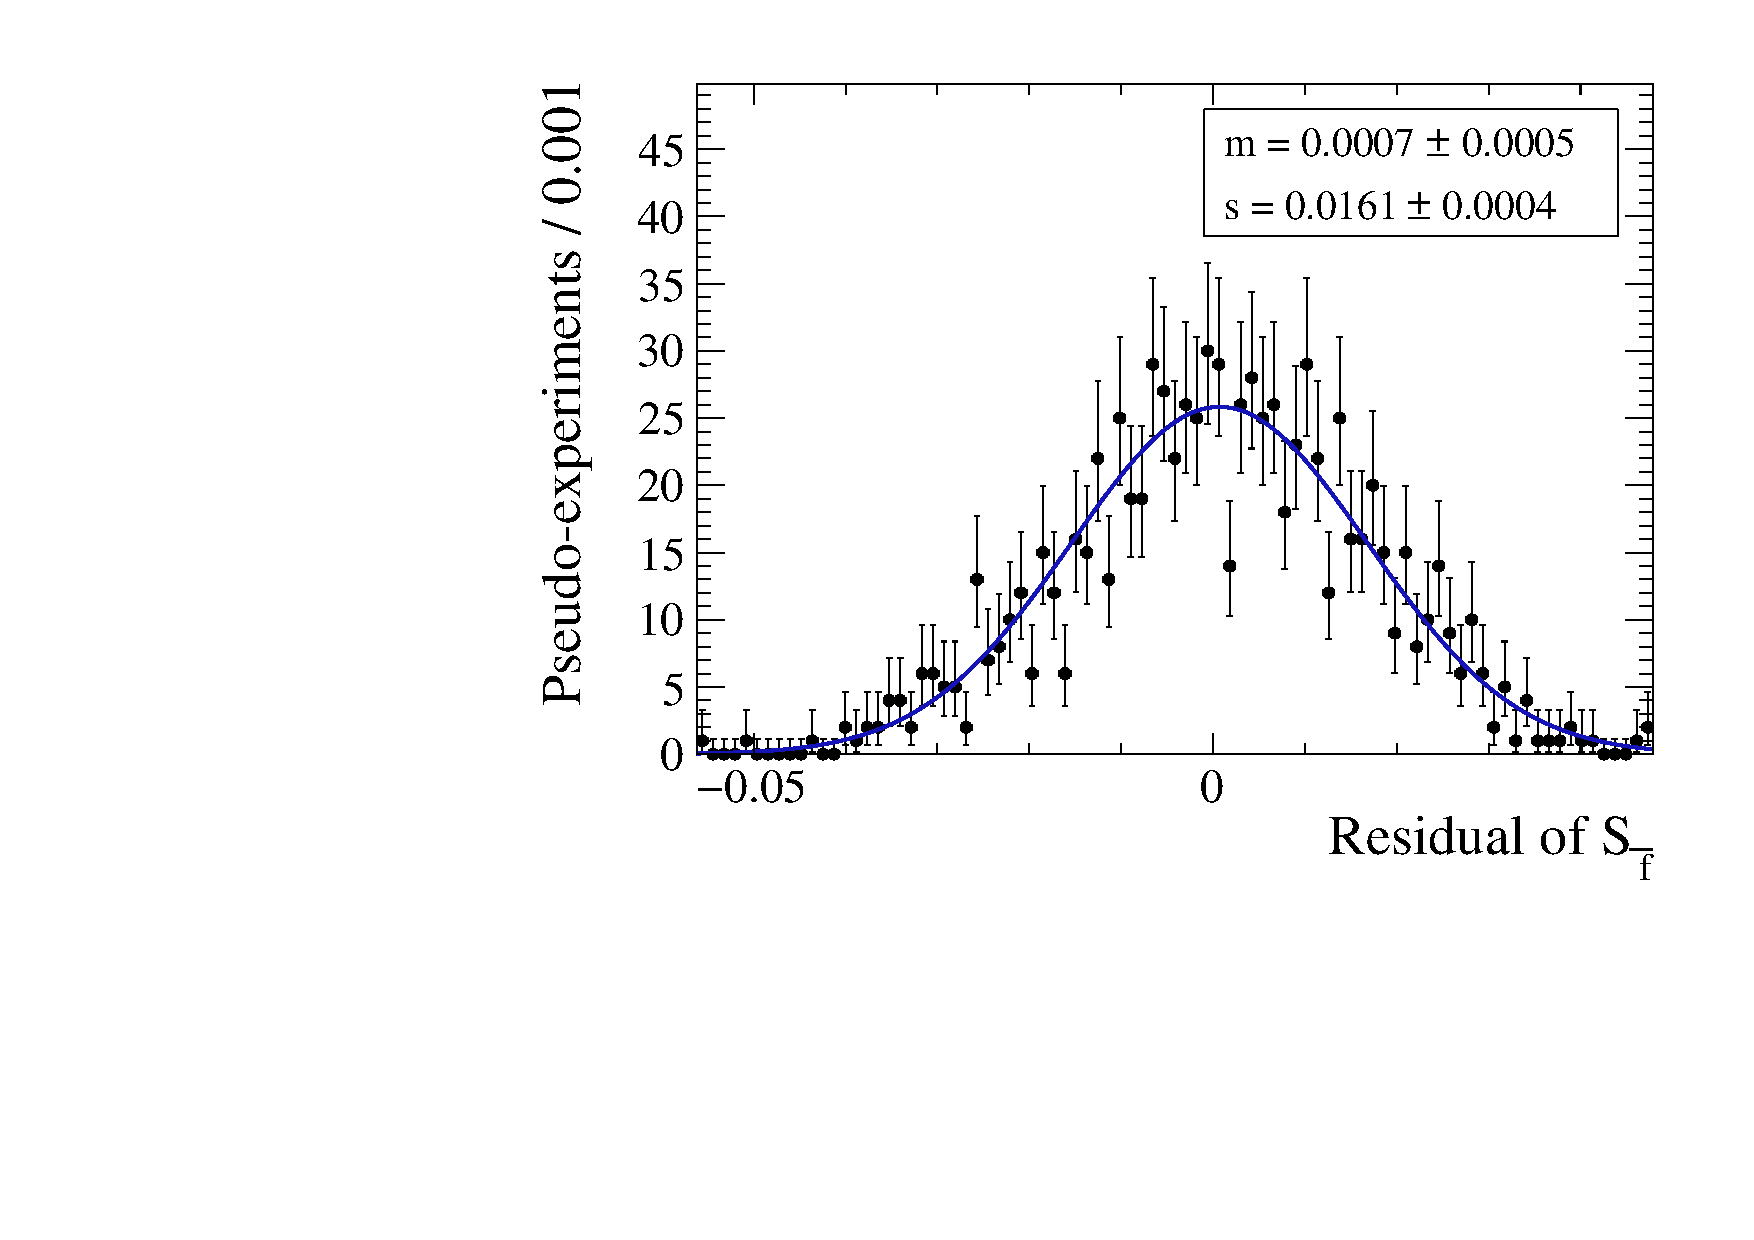
\includegraphics[width=0.48\textwidth]{10Systematics/figs/ResHigh_Sfbar_res.pdf}\\
    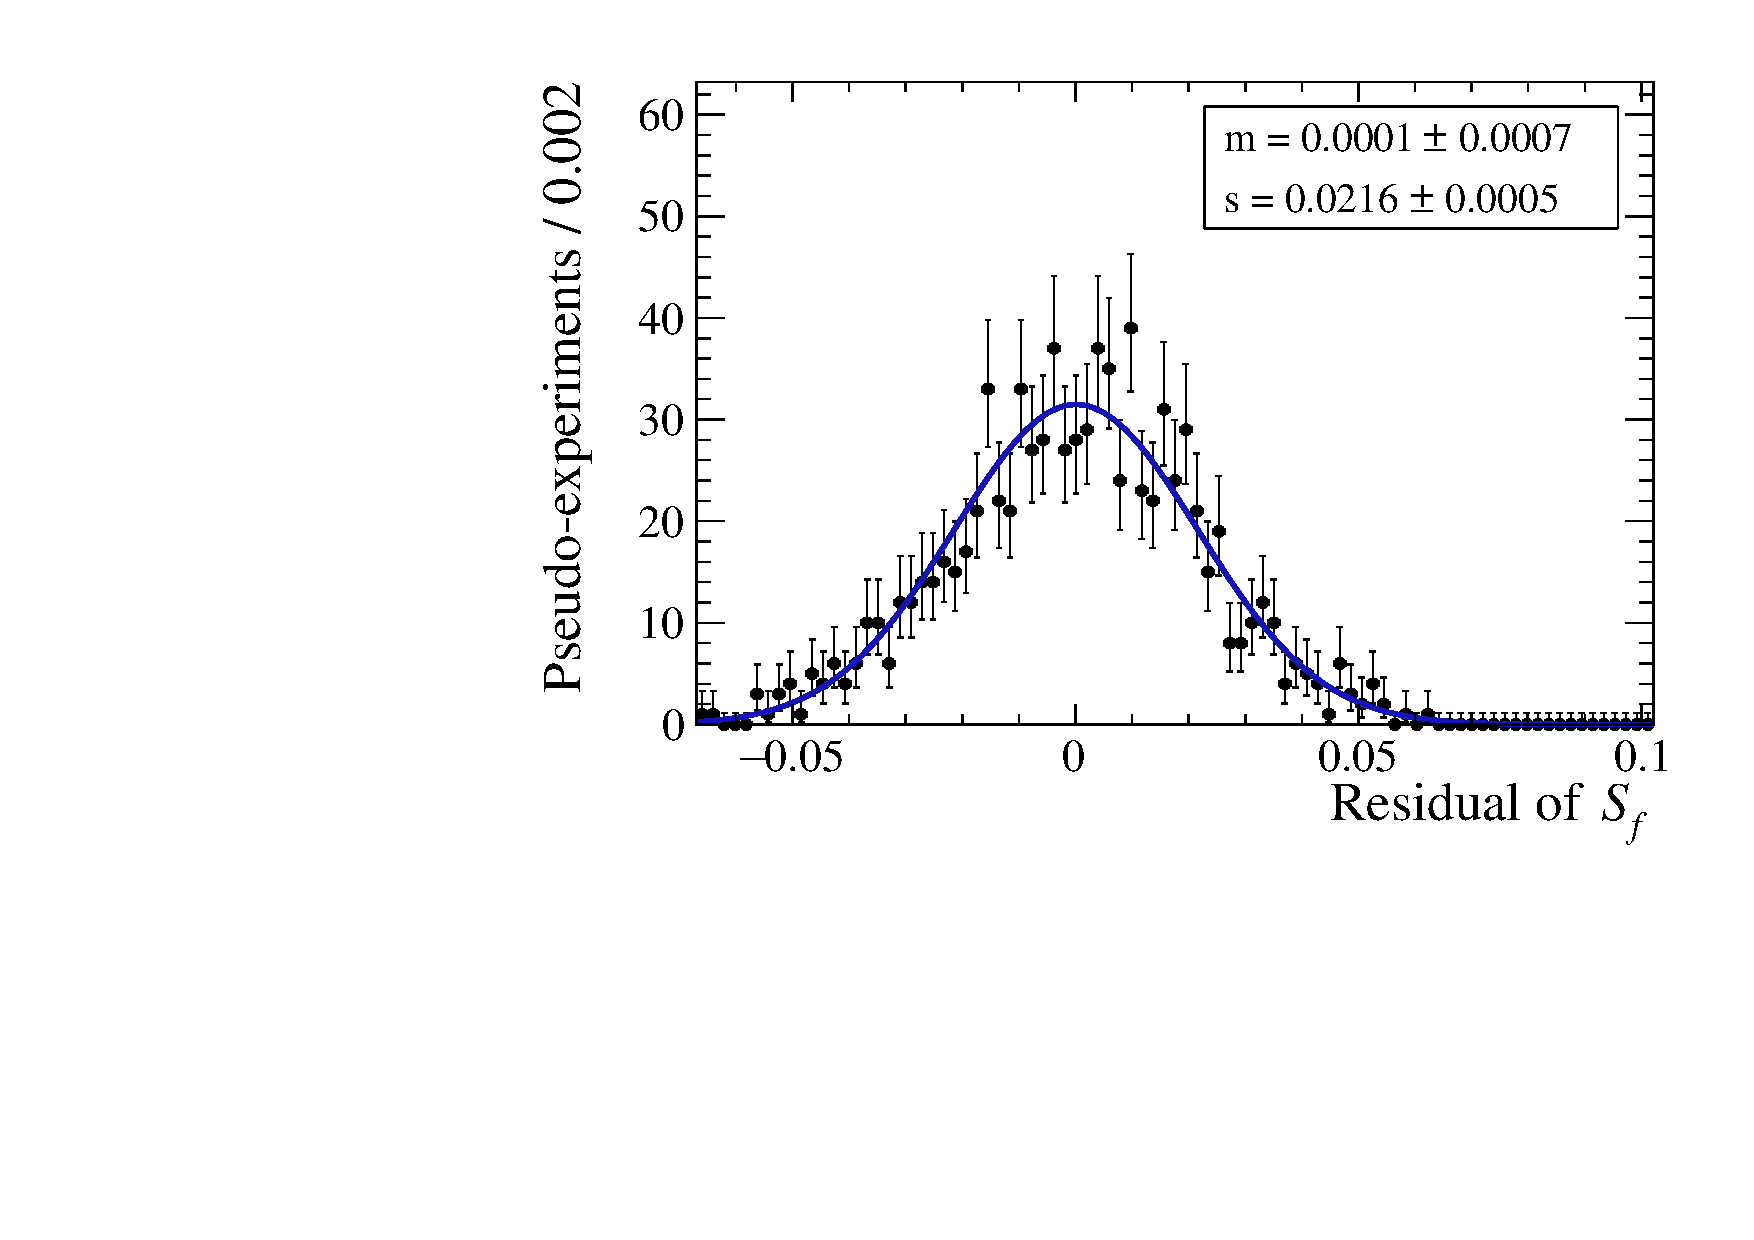
\includegraphics[width=0.48\textwidth]{10Systematics/figs/ResLow_Sf_res.pdf}
    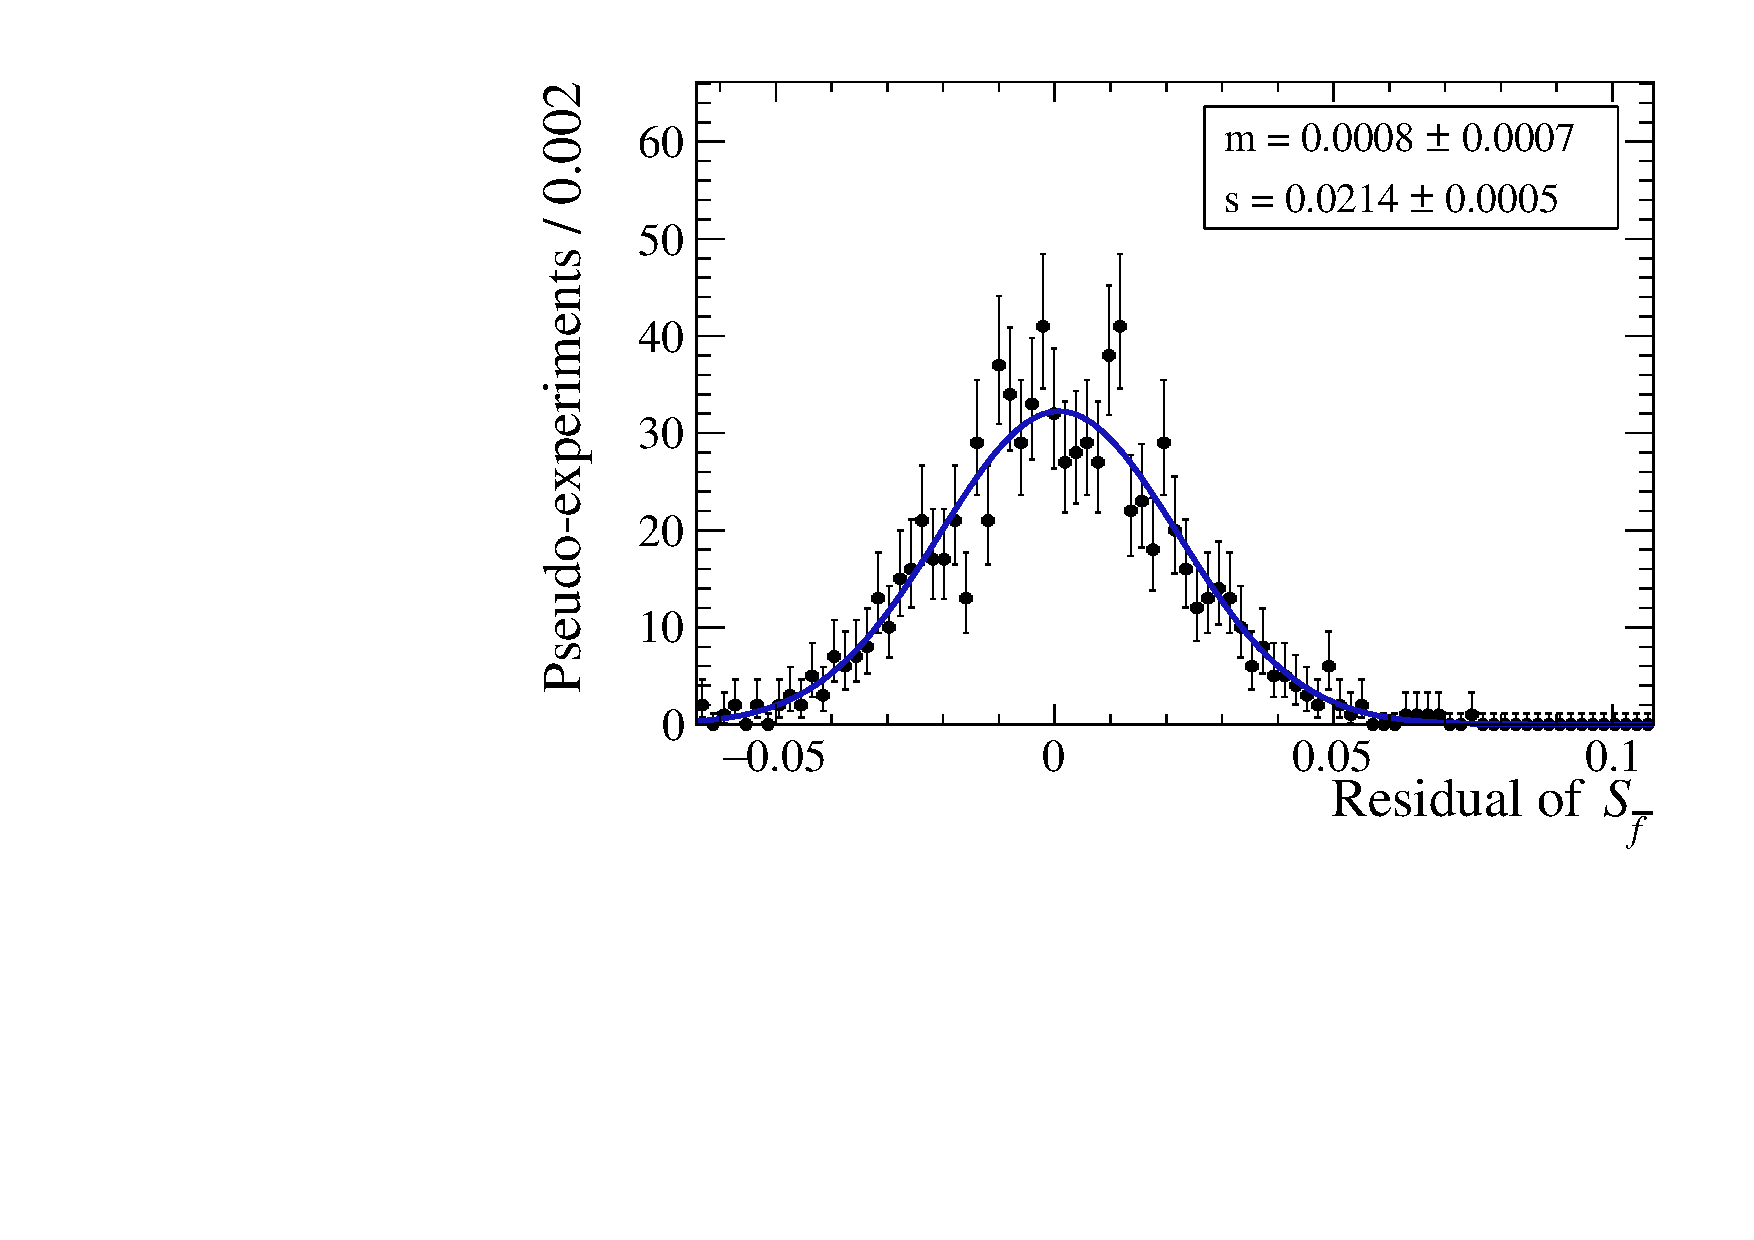
\includegraphics[width=0.48\textwidth]{10Systematics/figs/ResLow_Sfbar_res.pdf}
    \caption{Distribution of residuals for \Sf (left) and \Sfbar (right) to determine the systematic uncertainty due to the decay-time resolution.
    In the top  (bottom) row the resolution \SI{20}{\femto\second} higher (lower) than the nominal model is used.}
    \label{fig:systUncertRes}
\end{figure}

\subsection*{Acceptance model}

The samples of the pseudoexperiments are generated with the acceptance model presented in \cref{sec:acceptance}.
The model used in the fit has knots which are located at the following decay times: $[0.4, 0.5, 1.0, 1.5, 2.0, 2.3, 2.6, 3.0, 4.0, 10.0, 12.0]\,$\si{\pico\second}.
Hereby the tenth coefficient $v_{10}$ is set to one to fix the overall normalisation, and the eleventh coefficient is determined by a linear extrapolation of the two preceding coefficients (as stated in \cref{sec:acceptance}, this second model was developed by a collaborator).
The distributions of residuals for \Sf and \Sfbar are shown in \cref{fig:systUncertAcc}.
Since the mean values of the fitted distributions are compatible with zero, a systematic uncertainty of the uncertainty of the mean values of  \num{0.007} follows for both \CP parameters.
\begin{figure}[tbp]
    \centering
    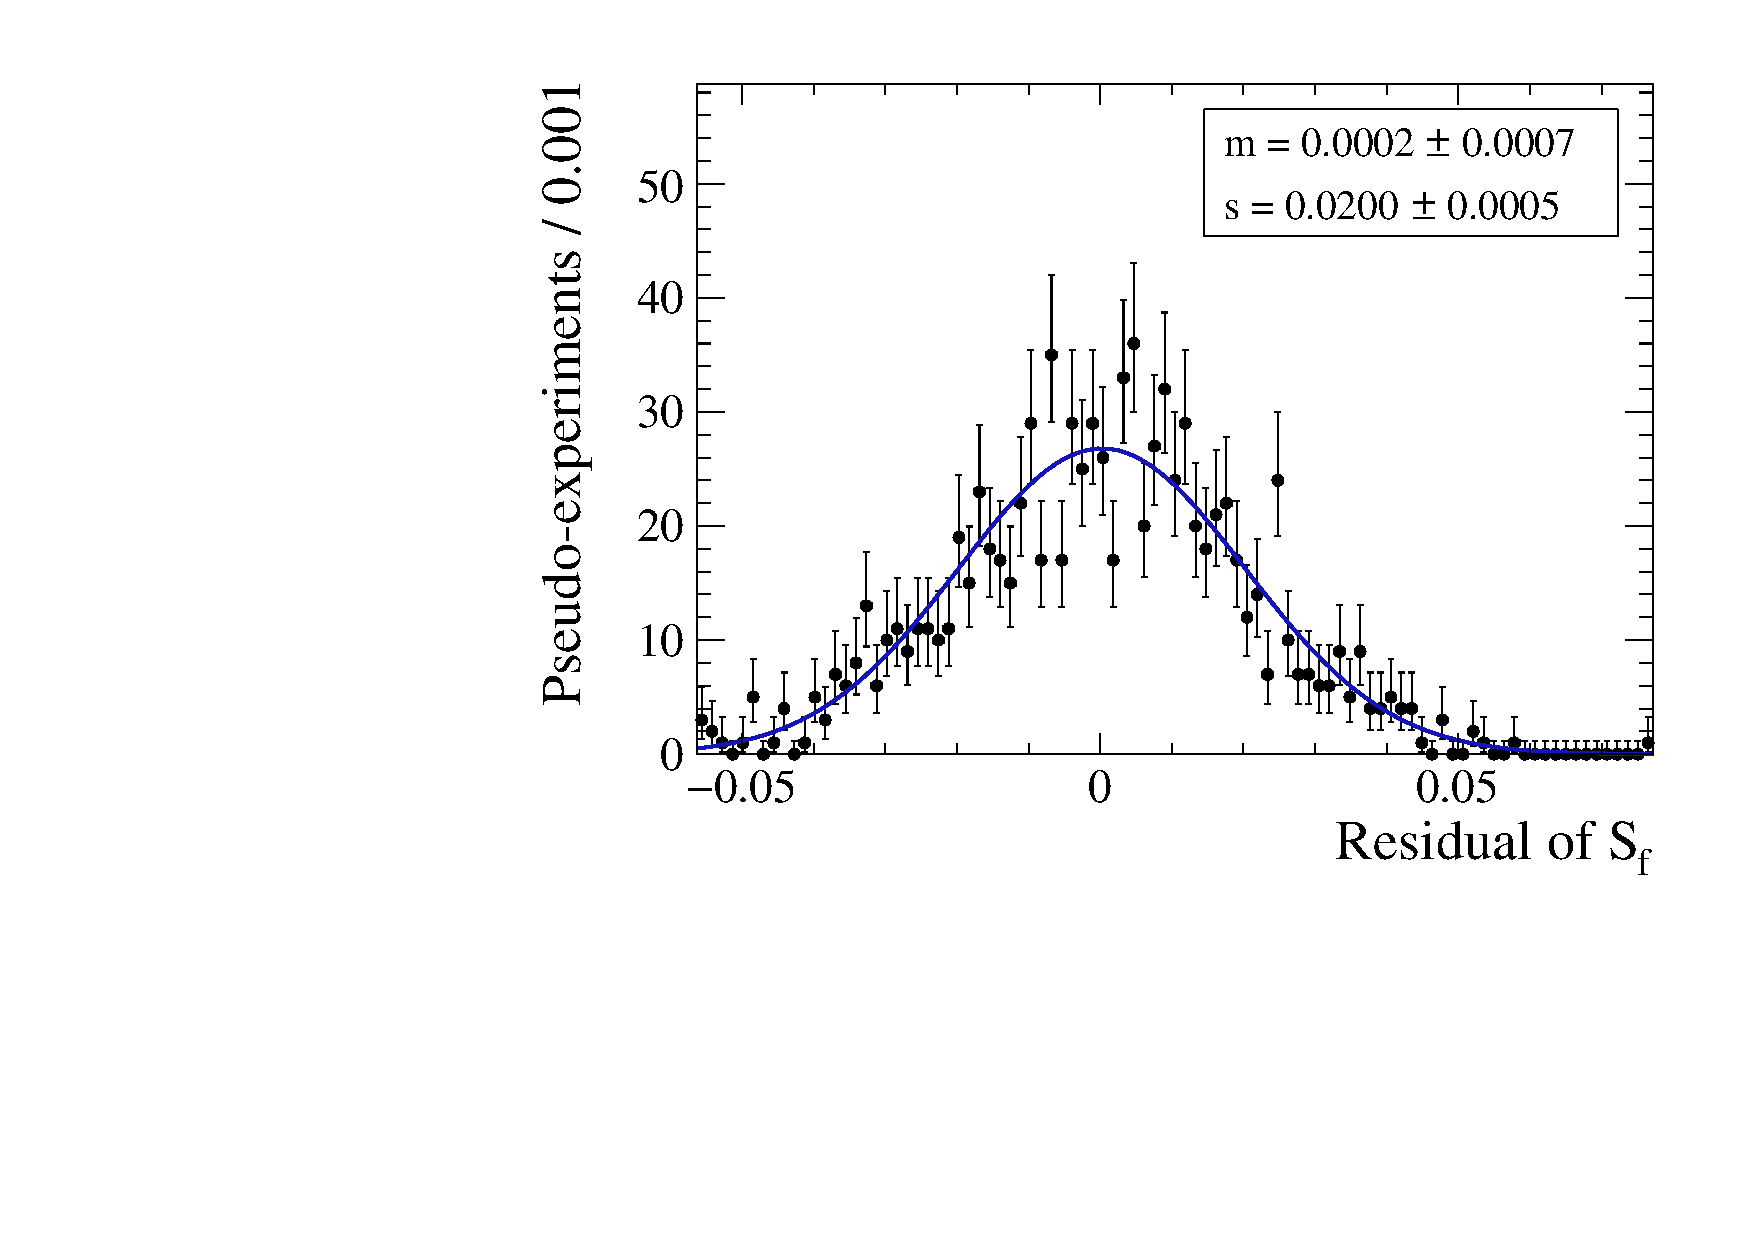
\includegraphics[width=0.48\textwidth]{10Systematics/figs/accept_Sf_res.pdf}
    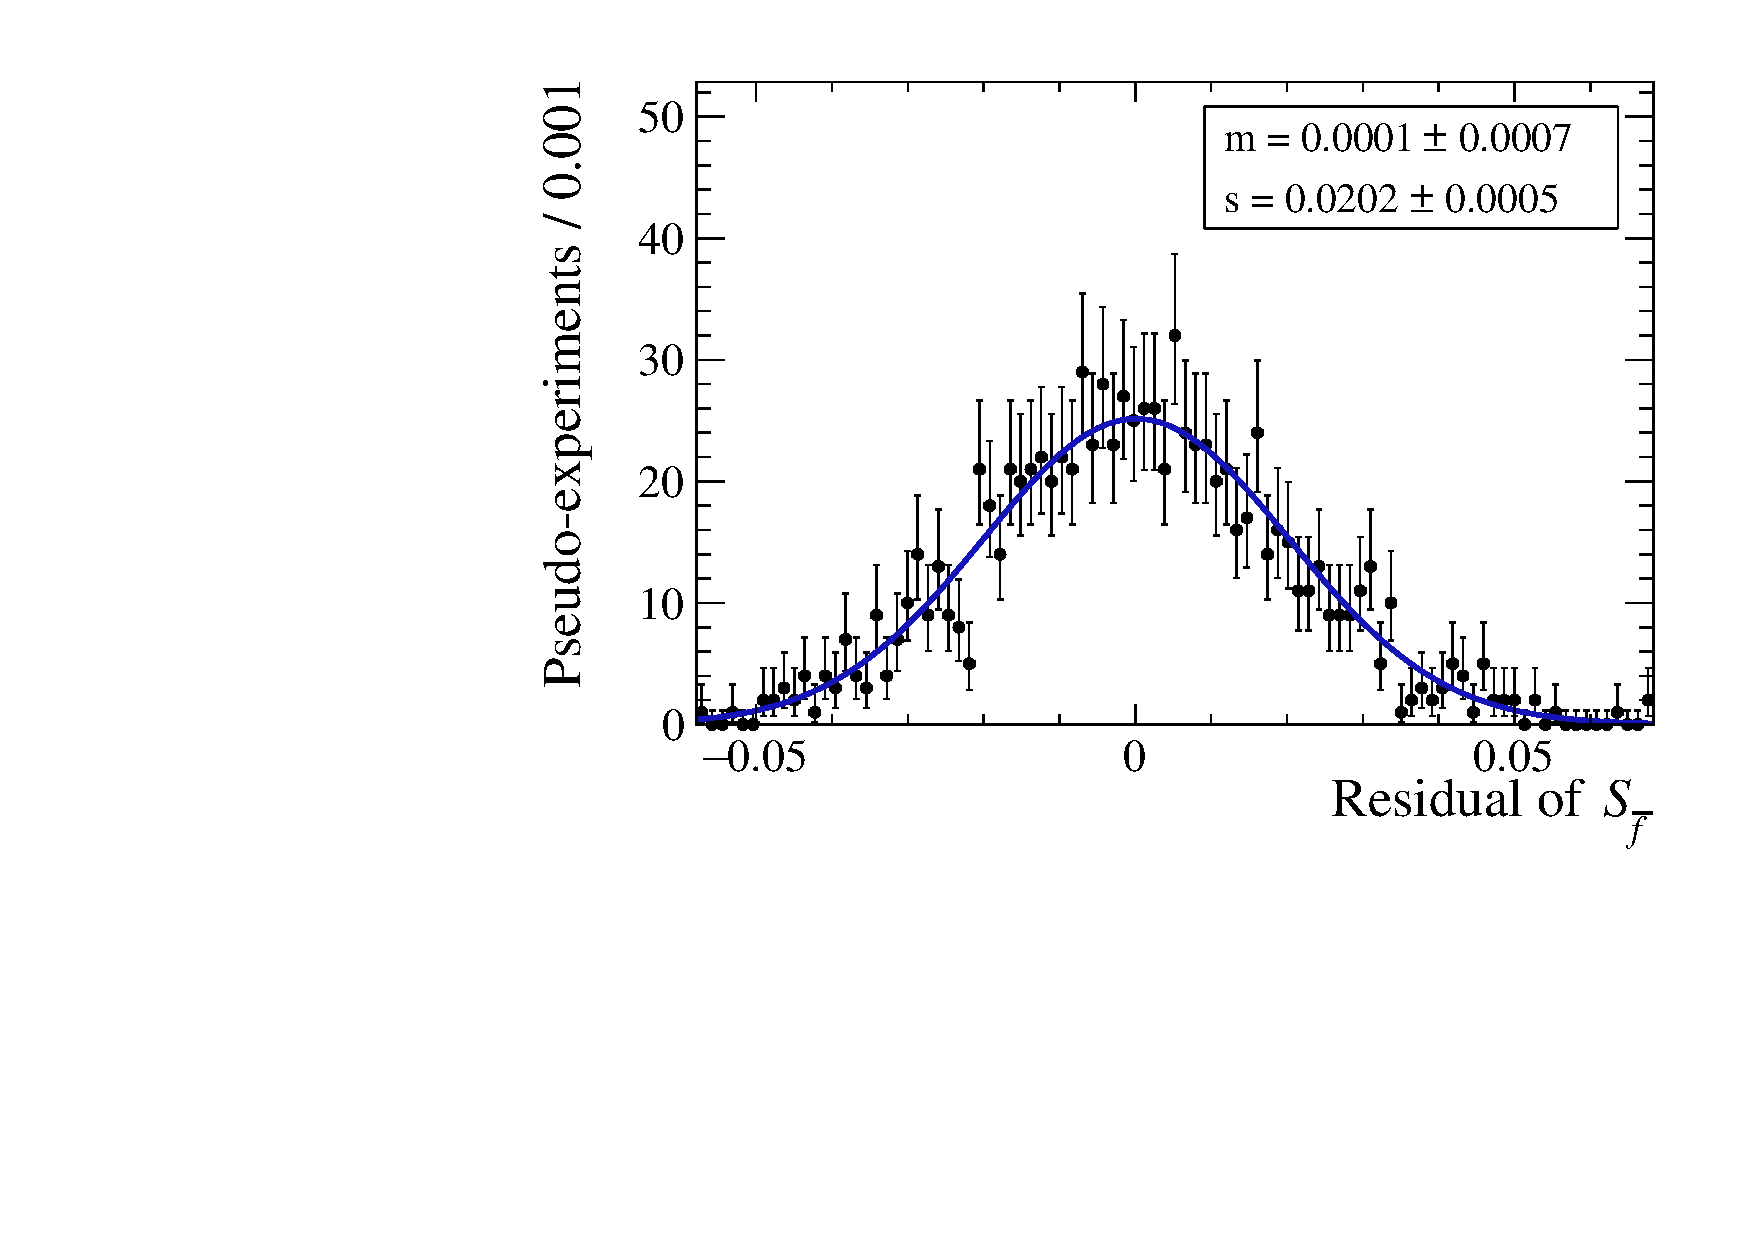
\includegraphics[width=0.48\textwidth]{10Systematics/figs/accept_Sfbar_res.pdf}
    \caption{Distribution of residuals for \Sf (left) and \Sfbar (right) to determine the systematic uncertainty due to the acceptance model.}
    \label{fig:systUncertAcc}
\end{figure}

\subsection*{Assumption on $\symbfsf{\DG}$}

The value of \DG is set to the world average plus one time its uncertainty in the generation, namely \SI{0.0079}{\per\pico\second}~\cite{HFLAV2016}.
Since the hyperbolic sine from \crefrange{eq:Ptof}{eq:Pbartofbar} does not vanish with $\DG\neq0$, the values for $A_f^{\DG}$ and $A_{\kern 1.5pt\overline{\kern -1.5pt f\kern 1.5pt}}^{\DG}$ need to be defined.
The same values as used in the generation of simulated events are used, namely \num{-0.0103} and \num{-0.0155}.
Then, the samples are fitted with the nominal strategy providing the residuals shown in \cref{fig:systUncertDG}.
As systematic uncertainty follows \num{0.0007} for both, \Sf and \Sfbar.
\begin{figure}[tbp]
    \centering
    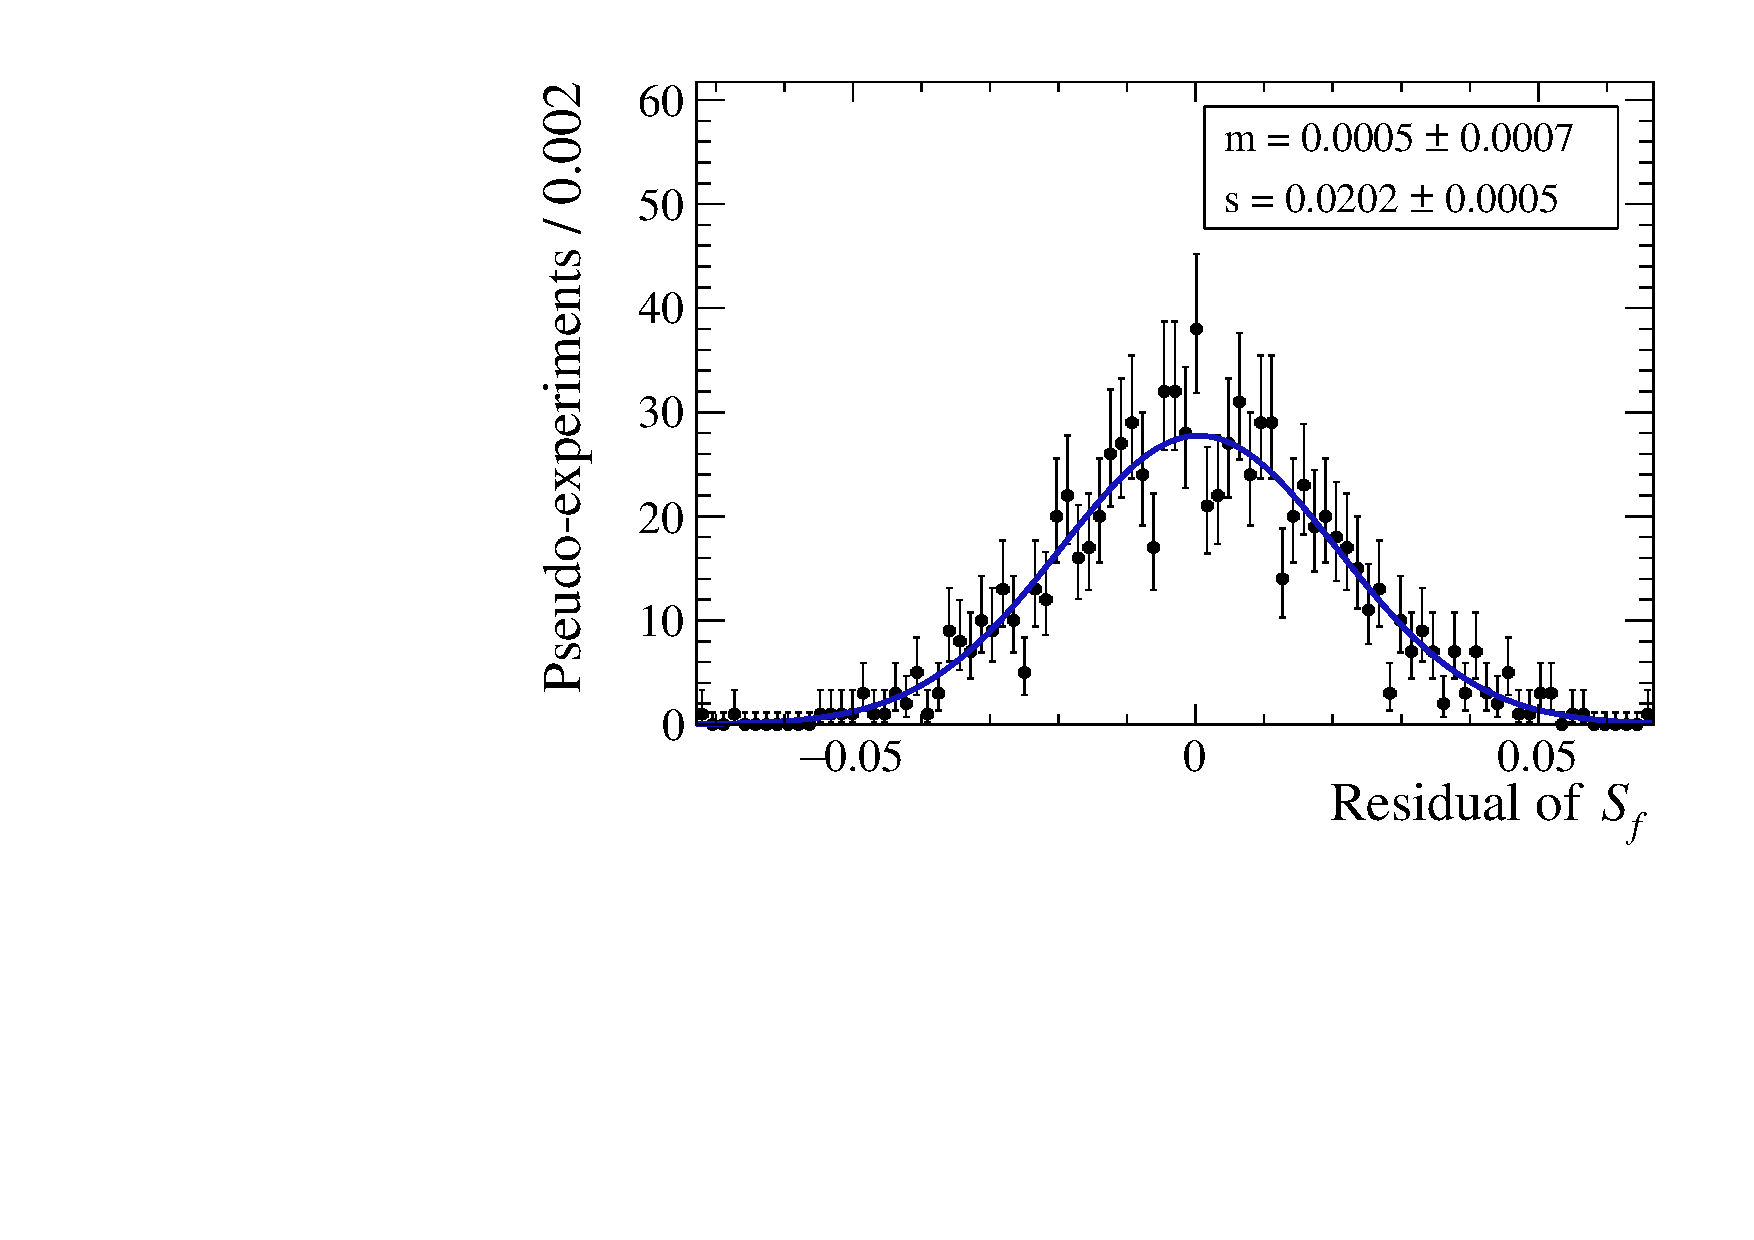
\includegraphics[width=0.48\textwidth]{10Systematics/figs/DG_Sf_res.pdf}
    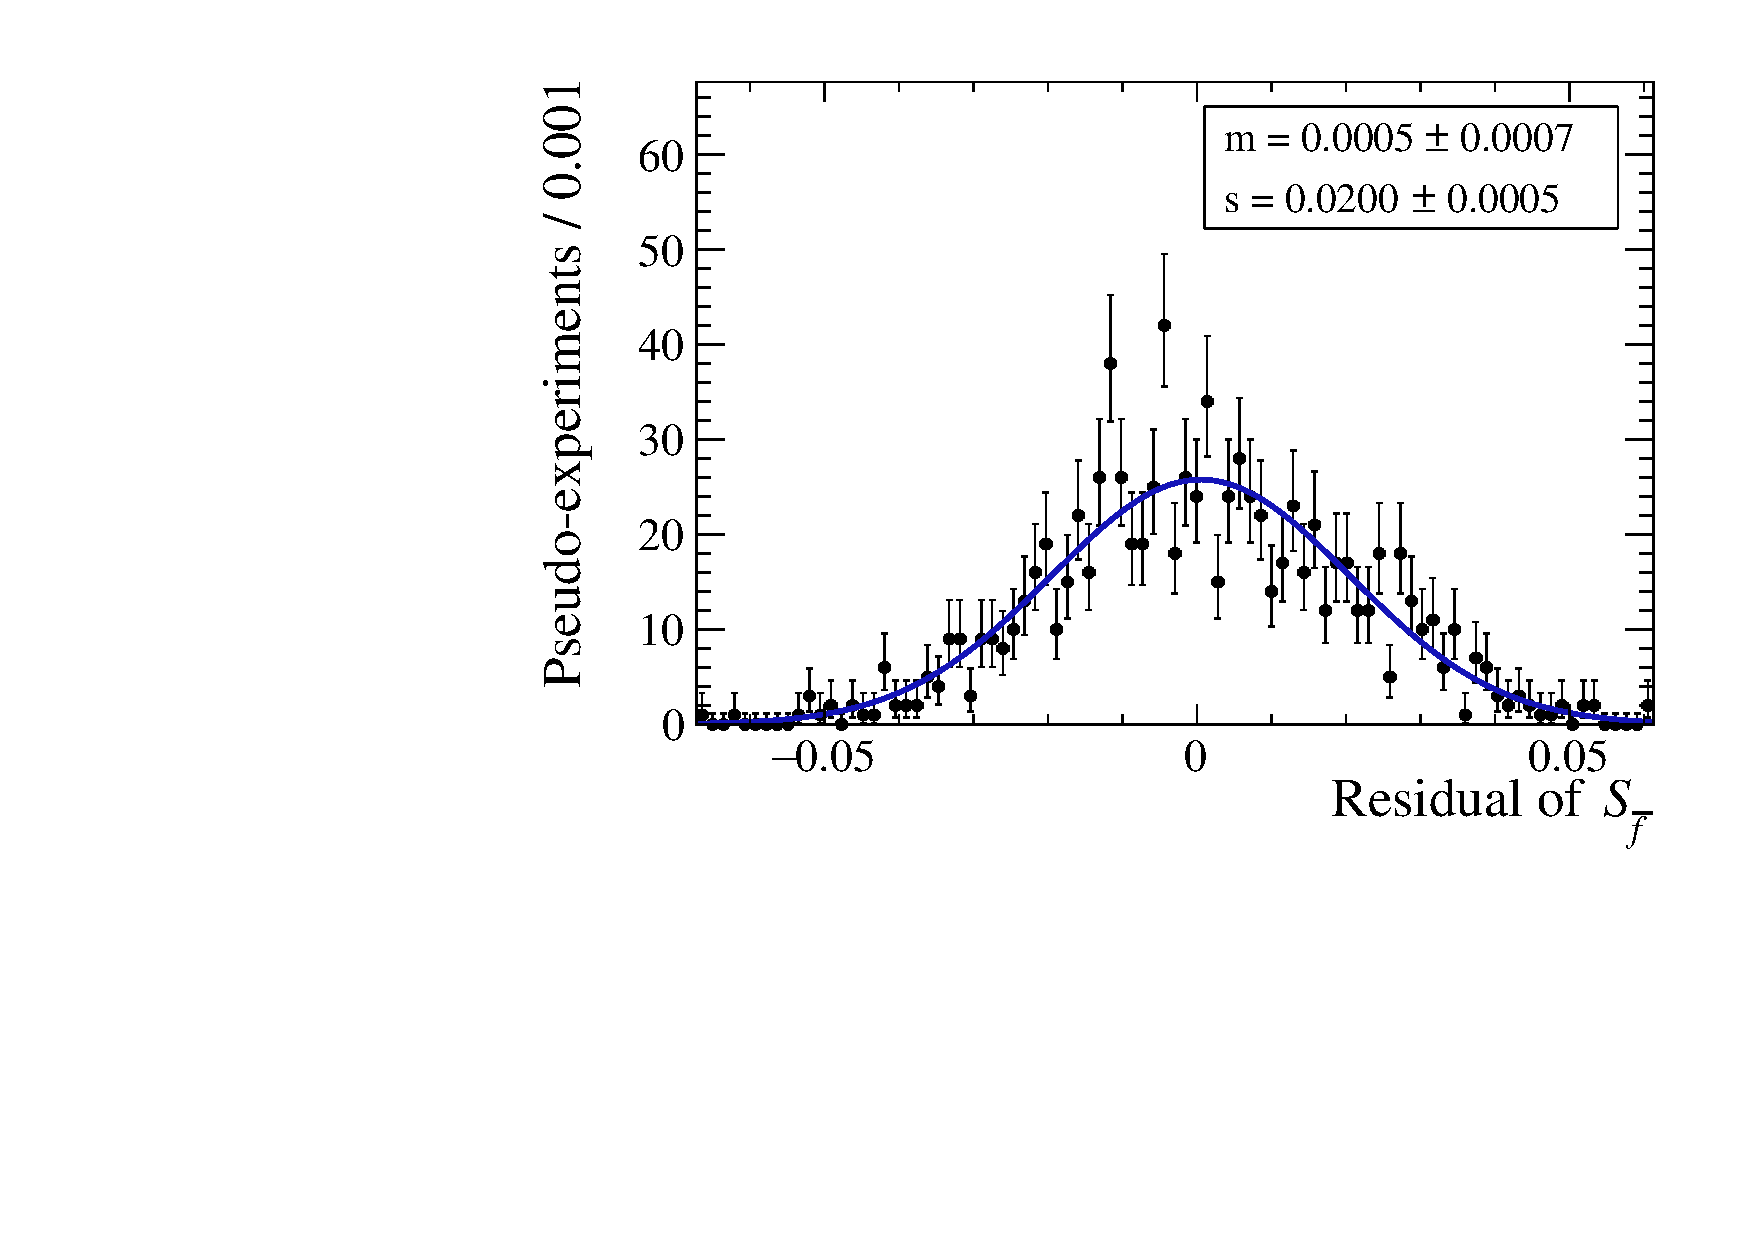
\includegraphics[width=0.48\textwidth]{10Systematics/figs/DG_Sfbar_res.pdf}
    \caption{Distribution of residuals for \Sf (left) and \Sfbar (right) to determine the systematic uncertainty due to the assumption on \DG.}
    \label{fig:systUncertDG}
\end{figure}

\subsection*{Assumption on $\symbfsf{\Cf}$}

In the generation, the values for \Cf and \Cfbar are calculated from the average measurements by \belle and \babar for the parameter $r$ plus the statistical uncertainty, namely 0.993~\cite{Aubert:2008zi, Das:2010be}.
In the Fit, \Cf and \Cfbar are then set to \num{1} and {-1} as in the nominal strategy.
The distribution of residuals for \Sf and \Sfbar is shown in \cref{fig:systUncertC} and provides \num{0.0006} as a systematic uncertainty for both parameters.
\begin{figure}[tbp]
    \centering
    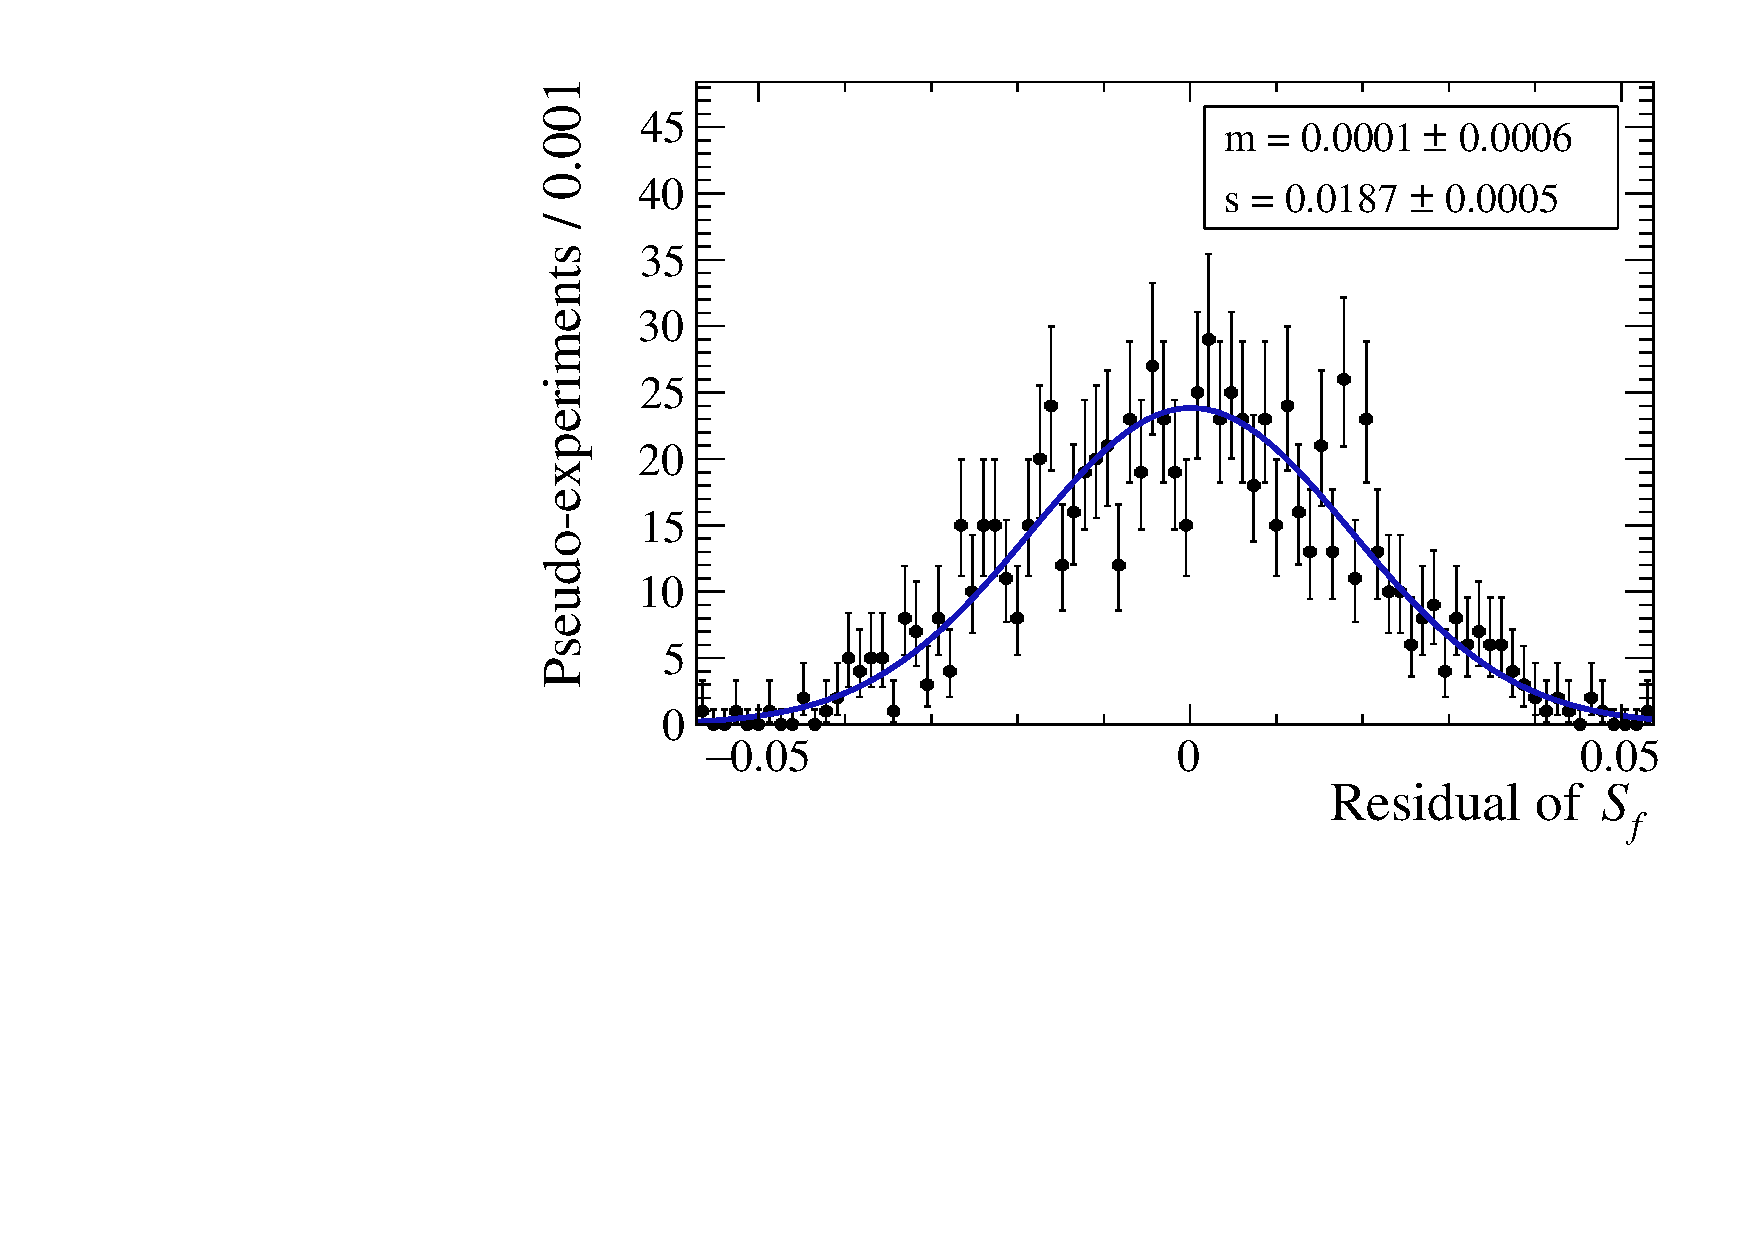
\includegraphics[width=0.48\textwidth]{10Systematics/figs/C_Sf_res.pdf}
    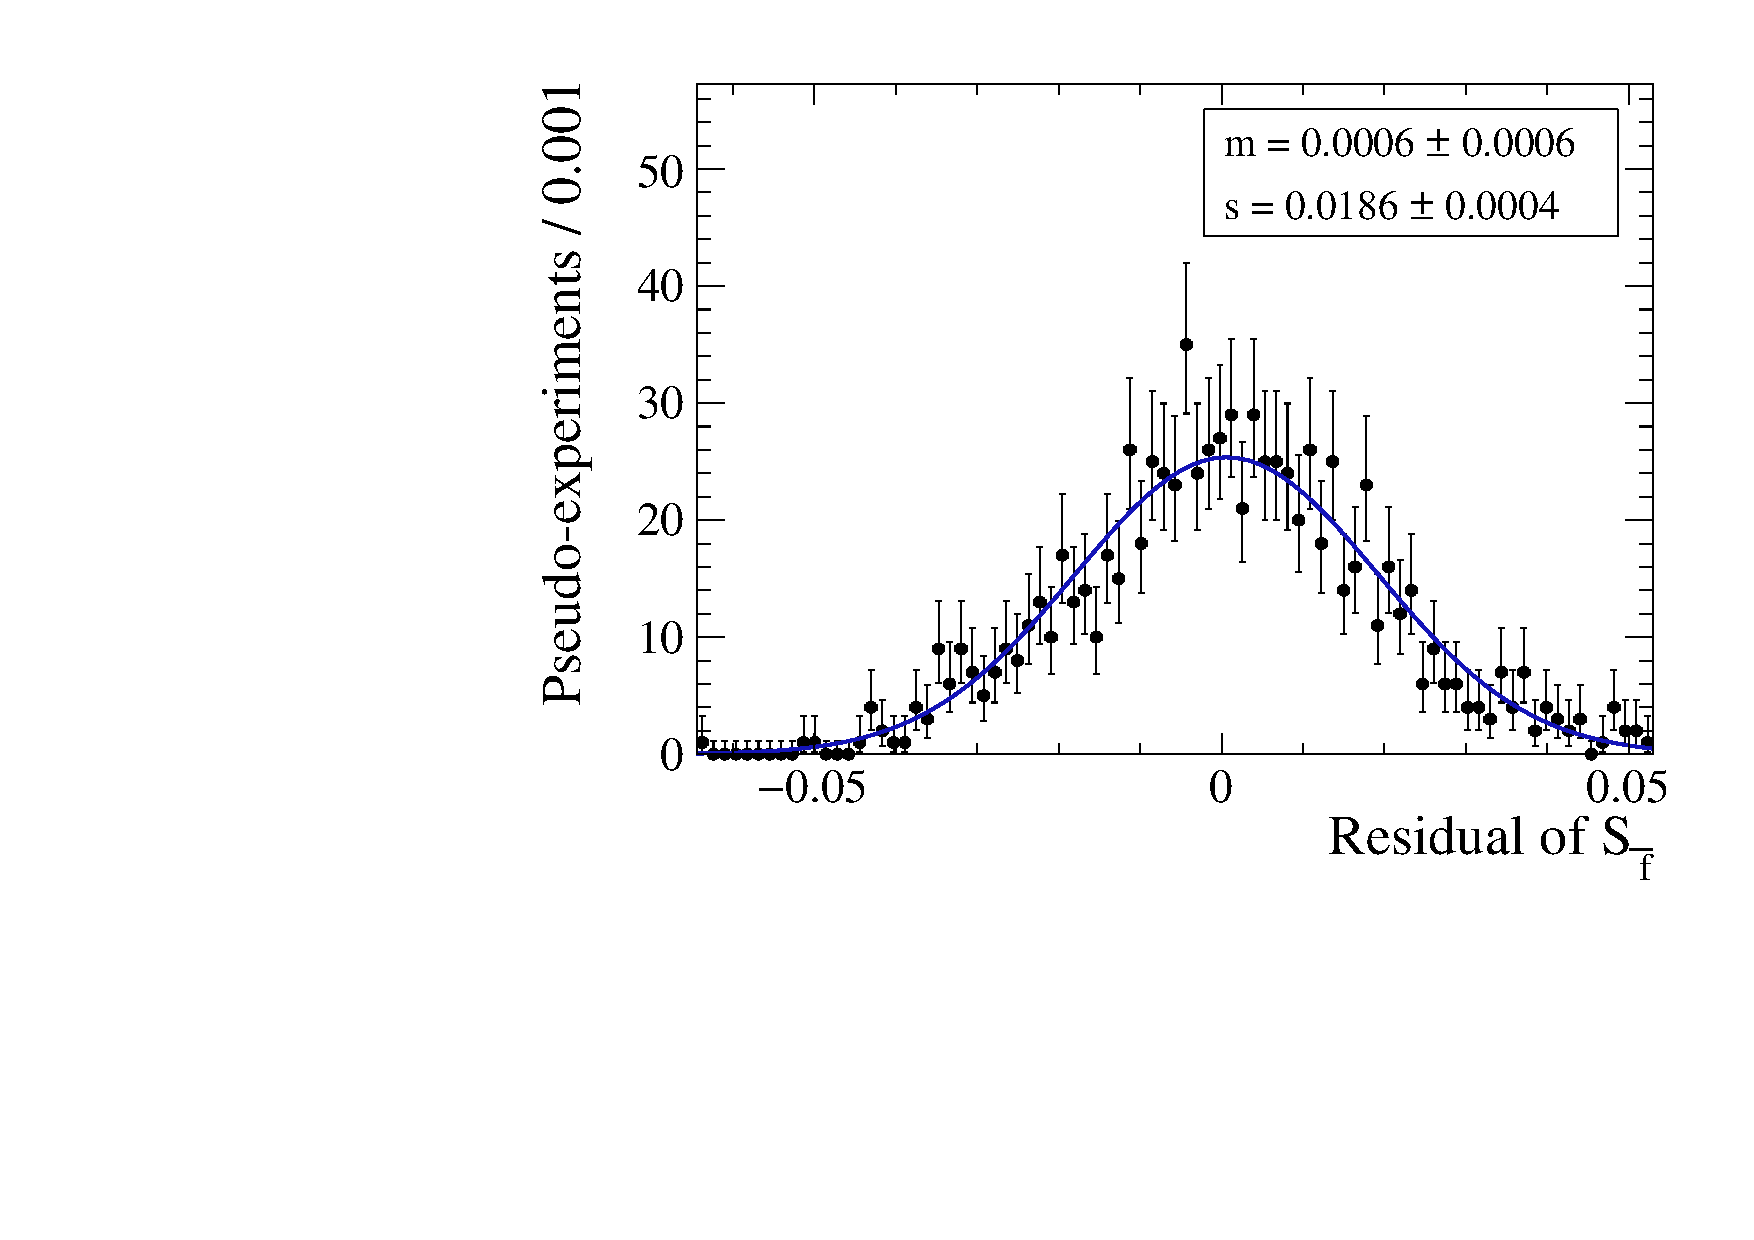
\includegraphics[width=0.48\textwidth]{10Systematics/figs/C_Sfbar_res.pdf}
    \caption{Distribution of residuals for \Sf (left) and \Sfbar (right) to determine the systematic uncertainty due to the assumption on \Cf and \Cfbar.}
    \label{fig:systUncertC}
\end{figure}

\section{Mass model}
\label{sec:SystUncertMass}

Before describing the estimation of systematic uncertainties due to mass parameterisation, it should again be mentioned that the studies related to this were completely carried out by a collaborator.

Since the model to describe the invariant mass is the essential ingredient for the calculation of the \emph{sWeights}, which are used in all subsequent steps of the analysis to make distributions look background subtracted, systematic effects from the parameterisation of the invariant mass can also influence the measurement of \Sf and \Sfbar.
To estimate a systematic uncertainty, the fit strategy, \ie the restriction of the invariant-mass range in Fit B, is checked.
For this purpose, Fit B is also performed in the wide range of the invariant mass, which leads to a larger background contamination in the subsequently used data sample.
With the \emph{sWeights} extracted from this fit, the decay-time fit is performed again.
The result shows a deviation of $2.3\sigma$ and $1.8\sigma$ for \Sf and \Sfbar, respectively.
Therefore, the difference between these newly obtained values and the nominal results for \Sf and \Sfbar parameters is taken as systematic uncertainty, namely \num{0.0042} and \num{0.0023}.
Additionally a second test to check the strategy of splitting of the data sample in order to control the $\Bu\!\to\Dm\Kp$ component is performed.
This test yields a good agreement of $0.4\sigma$ and $1.5\sigma$ for \Sf and \Sfbar, respectively, and therefore no additional systematic uncertainty is assigned, especially given the fact that a systematic uncertainty concerning the requirement on \dllkpi is already assigned in \cref{sec:SystUncertsGauss}.

As a last test, the fit of the invariant mass as a tool to subtract the background is simply \enquote{replaced} by a narrow mass range of $[5250,5330]\,$\si[per-mode=symbol]{\MeVcc}, \ie no \emph{sWeights} are calculated.
This is possible due to the high purity in the signal range,
The decay-time fit is then performed on a data sample containing both, signal and backgrounds which are distributed under the signal peak in the invariant mass distribution.
The agreement between the nominal result and the result obtained without \emph{sWeights} is $0.2\sigma$ and $1.3\sigma$ for \Sf and \Sfbar, respectively.
Due to this good agreement, despite the extreme test without any background suppression in the signal range, no further systematic uncertainty is assigned.
